


\tikzset{every picture/.style={line width=0.75pt}} %set default line width to 0.75pt

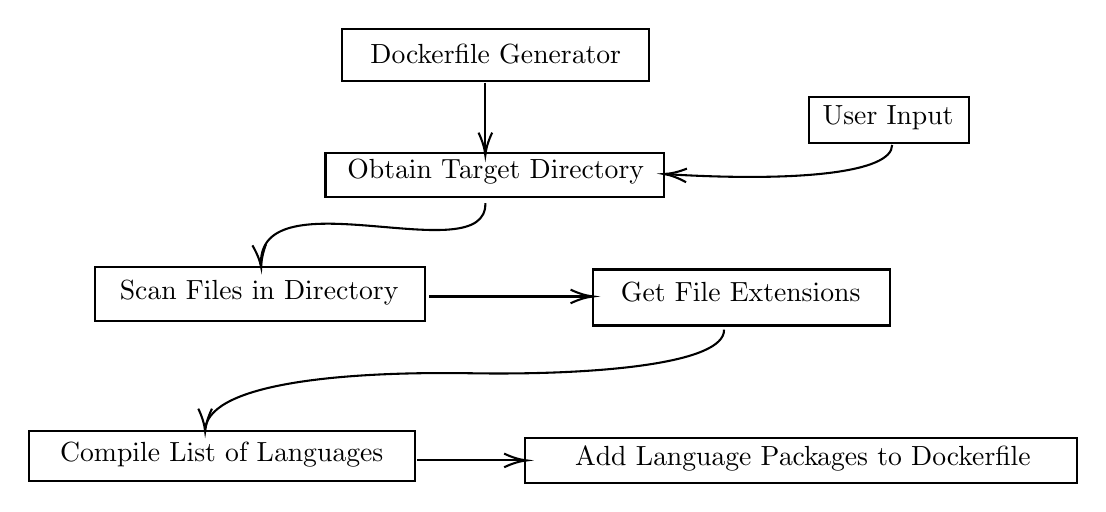
\begin{tikzpicture}[x=0.75pt,y=0.75pt,yscale=-1,xscale=1]
%uncomment if require: \path (0,447); %set diagram left start at 0, and has height of 447

%Shape: Rectangle [id:dp6708330246204339]
\draw   (254,19) -- (402,19) -- (402,44) -- (254,44) -- cycle ;
%Shape: Rectangle [id:dp3690663496827087]
\draw   (246,79) -- (409,79) -- (409,100) -- (246,100) -- cycle ;
%Shape: Rectangle [id:dp04032174080708906]
\draw   (479,52) -- (556,52) -- (556,74) -- (479,74) -- cycle ;
%Shape: Rectangle [id:dp3663336326705653]
\draw   (135,134) -- (294,134) -- (294,160) -- (135,160) -- cycle ;
%Shape: Rectangle [id:dp1296990044512687]
\draw   (375,135) -- (518,135) -- (518,162) -- (375,162) -- cycle ;
%Shape: Rectangle [id:dp5900699675454877]
\draw   (103,213) -- (289,213) -- (289,237) -- (103,237) -- cycle ;
%Shape: Rectangle [id:dp5669318997590742]
\draw   (342,216) -- (608,216) -- (608,238) -- (342,238) -- cycle ;
%Straight Lines [id:da9499154626346906]
\draw    (323,45) -- (323,78) ;
\draw [shift={(323,80)}, rotate = 270] [color={rgb, 255:red, 0; green, 0; blue, 0 }  ][line width=0.75]    (10.93,-3.29) .. controls (6.95,-1.4) and (3.31,-0.3) .. (0,0) .. controls (3.31,0.3) and (6.95,1.4) .. (10.93,3.29)   ;
%Curve Lines [id:da07473585010478478]
\draw    (519,75) .. controls (519,88.37) and (473.92,92.91) .. (410.91,89.12) ;
\draw [shift={(409,89)}, rotate = 363.58000000000004] [color={rgb, 255:red, 0; green, 0; blue, 0 }  ][line width=0.75]    (10.93,-3.29) .. controls (6.95,-1.4) and (3.31,-0.3) .. (0,0) .. controls (3.31,0.3) and (6.95,1.4) .. (10.93,3.29)   ;
%Curve Lines [id:da3255234731100256]
\draw    (323,103) .. controls (323.99,136.66) and (213.25,88.97) .. (214.91,132.65) ;
\draw [shift={(215,134)}, rotate = 265.03] [color={rgb, 255:red, 0; green, 0; blue, 0 }  ][line width=0.75]    (10.93,-3.29) .. controls (6.95,-1.4) and (3.31,-0.3) .. (0,0) .. controls (3.31,0.3) and (6.95,1.4) .. (10.93,3.29)   ;
%Straight Lines [id:da9168787921818711]
\draw    (296,148) -- (373,148) ;
\draw [shift={(375,148)}, rotate = 180] [color={rgb, 255:red, 0; green, 0; blue, 0 }  ][line width=0.75]    (10.93,-3.29) .. controls (6.95,-1.4) and (3.31,-0.3) .. (0,0) .. controls (3.31,0.3) and (6.95,1.4) .. (10.93,3.29)   ;
%Curve Lines [id:da18630293162808487]
\draw    (438,164) .. controls (438.48,180.4) and (377,186) .. (316,185) .. controls (256.52,184.03) and (191.35,189.42) .. (188.12,211.29) ;
\draw [shift={(188,213)}, rotate = 270] [color={rgb, 255:red, 0; green, 0; blue, 0 }  ][line width=0.75]    (10.93,-3.29) .. controls (6.95,-1.4) and (3.31,-0.3) .. (0,0) .. controls (3.31,0.3) and (6.95,1.4) .. (10.93,3.29)   ;
%Straight Lines [id:da8834662262571595]
\draw    (290,227) -- (341,227) ;
\draw [shift={(343,227)}, rotate = 180] [color={rgb, 255:red, 0; green, 0; blue, 0 }  ][line width=0.75]    (10.93,-3.29) .. controls (6.95,-1.4) and (3.31,-0.3) .. (0,0) .. controls (3.31,0.3) and (6.95,1.4) .. (10.93,3.29)   ;

% Text Node
\draw (328,31) node   [align=left] {Dockerfile Generator};
% Text Node
\draw (328,88) node   [align=left] {Obtain Target Directory};
% Text Node
\draw (517,62) node   [align=left] {User Input};
% Text Node
\draw (214,146) node   [align=left] {Scan Files in Directory};
% Text Node
\draw (446,146) node   [align=left] {Get File Extensions};
% Text Node
\draw (196,224) node   [align=left] {Compile List of Languages};
% Text Node
\draw (476,226) node   [align=left] {Add Language Packages to Dockerfile};


\end{tikzpicture}
